% !TeX root = Stageportfolio.tex



\begin{landscape}
	\subsubsection{Les 16}
	\begin{tabularx}{1.56\textwidth}{|p{0.35\textwidth}|X|}\hline
		\textbf{Administratieve gegevens}\newline\newline
		Kevin Truyaert\newline\newline
		technisch secundair onderwijs\newline
		3e graad, 1ste jaar, Techniek-Wetenschappen\newline
		VVKSO: \href{http://ond.vvkso-ict.com/leerplannen/doc/Toegepaste\%20fysica-2014-041.pdf}{http://ond.vvkso-ict.com/leerplannen /doc/Toegepaste\%20fysica-2014-041.pdf} \newline
		\underline{Lesonderwerp}:\newline Bespreking labo M4\& De wet van Lenz invullen \& algemene inductiewet: Faraday-Lenz + oefeningen & \textbf{Doelstellingen}
		\begin{itemize}[itemsep=0.08\baselineskip]
			\item B27: Fluxverandering als oorzaak van inductiespanning toelichten
			\item B28: Met behulp van de wet van Lenz de zin van de inductiespanning vinden
			\item B29: De algemene inductiewet hanteren.
		\end{itemize}
		\underline{Lesdoelen}\newline
		\vspace{-0.75cm}
		\begin{enumerate}[itemsep=0.08\baselineskip]
			\item De leerlingen kunnen de zin van de inductiestroom bepalen.
			\item De leerlingen kunnen de wet van Lenz verwoorden.
			\item De leerlingen kunnen de samenhang tussen de wet van Faraday en de wet van Lenz uitleggen.
			\item De leerlingen kunnen de wet van Faraday-Lenz reproduceren.
			\item De leerlingen kunnen de wet van Faraday-Lenz op een rechte, bewegende geleider toepassen.
			\item De leerlingen kunnen de algemene inductiewet tijdens oefeningen hanteren.
		\end{enumerate} \\\hline
	\end{tabularx}\vfill \textcolor{white}{.} 


	\begin{tabularx}{1.56\textwidth}{|p{0.55\textwidth}|X|}
		\hline
		\multirow{2}{0.55\textwidth}{\textbf{Beginsituatie}\newline  
		Er zijn acht leerlingen binnen 5TW. Er heerst een algemene klassfeer. De leerlingen hebben al theorie gekregen  rond en oefeningen gemaakt op de magnetische krachtwerking. \newline\newline De leerlingen hebben vorige week de wet van Faraday en Lenz gezien. Hiermee kunnen ze de grootte en de zin van de inductiespanning bepalen. Ook met de begrippen flux en fluxverandering zijn ze gekend. \newline\newline Vorige les heb ik uitgebreide feedback van zowel de vakmentor als de stage begeleider verkregen. Deze wil ik in deze en komende lessen proberen te integreren. De grootste bemerking waar ik rekening mee wil houden is dat ik nog meer van de leerlingen zelf mag laten komen, door hen bijvoorbeeld aan bord oefeningen te laten bespreken.} & \textbf{Acties}\newline\newline %Vandaag worden de belangrijkste aspecten hiervan nog even overlopen. Daarnaast zijn we gisteren ook begonnen aan een nieuw stuk theorie rond elektromagnetische inductie. Hiervan hebben we de basis rond magnetische flux al besproken. Dit wordt nog even terug aangehaald.
		- \GreenHighlight{Via demo's wil ik bepaalde onderwerpen starten.}{9cm}	Op die manier kan ik de interesse van de leerlingen wekken en kan ik fysische wetmatigheden hen effectief aantonen. Zo kunnen leerlingen op een klassikale manier zelfstandig dingen ontdekken.	 \newline\newline 
		- Ik wil oefeningen op zo'n wijze brengen dat ze steeds dezelfde structuur hebben. Die structuur bouw ik eerst samen met de leerlingen op, om ze daarna zelfstandig aan de slag te laten gaan met oefeningen die steeds wat complexer worden. \PinkHighlight{Tijdens het zelfstandig maken van de oefeningen probeer ik toch zeker}{13cm} \PinkHighlight{de zwakkere leerlingen in de gaten te houden en hen individueler te coachen bij het}{15cm} \PinkHighlight{maken van oefeningen.}{4.5cm}
		Bij het maken van die oefeningen zal ik de leerlingen wat meer zelf laten doen.
		\newline\newline\newline\newline
		
		\\ \cline{2-2}
		  & \textbf{Bronnen}\begin{itemize}
		  	\item Schramme, S. (2018-2019) Cursus hoofdstuk 5: elektromagnetische inductie
		  	\item Giancoli, D. C. (2008). Physics for scientists and engineers. Pearson Education International.
		  \end{itemize}\\ \hline
	\end{tabularx}


\newpage
	


\begin{tabularx}{1.56\textwidth}{|p{1.5cm}|p{8cm}|X|p{4cm}|}
	\hline
	\textbf{Nr. lesdoel } & \textbf{Inhoud (timing)}  & \textbf{Organisatie } & \textbf{Media } \\ \hline
	1\newline\newline 2&\underline{De wet van Lenz (10 minuten)}\newline
	Invullen pagina 11\& 12 gebeurde thuis nadat de demo uitvoerig besproken geweest is tijdens vorige les: nu overlopen + eventuele vragen van de leerlingen bespreken
	&  \underline{Onderwijsleergesprek}\newline 
	Projectie: figuur pagina 11 = weergave demo\newline
	Bespreken pagina's 11 en 12\newline
	Aandachtspunt: nogmaals hameren dat fluxverandering de oorzaak is door:
	\begin{itemize}
		\item vraag hen wat essentieel is voor inductiespanning
		\item Hoe ontstaat fluxverandering?
	\end{itemize}
	&   Cursus hoofdstuk 5 p11-12\newline\newline Krijtbord + projectie \newline\newline Elekromagneet, weekijzeren kern, hangende ring
	\\ \hline
\end{tabularx}\vspace{5mm}

	
\begin{tabularx}{1.56\textwidth}{|p{1.5cm}|p{8cm}|X|p{4cm}|}
	\hline
	\textbf{Nr. lesdoel } & \textbf{Inhoud (timing)}  & \textbf{Organisatie } & \textbf{Media } \\ \hline
	2\newline\newline 3\newline\newline &\underline{De algemene inductiewet:} \underline{Faraday-Lenz (5 minuten)}\newline
	De wet van Faraday-Lenz = combinatie van de wet van Faraday en de wet van Lenz.
	&  \underline{Onderwijsleergesprek}\newline 
	Bespreken van de wet:\newline
	$U_i(t) = -N\cdot\frac{\Delta \Phi}{\Delta t}$ Welke termen komen uit Faraday, welke uit Lenz? Wat vertelt dit juist opnieuw?
	&   Cursus hoofdstuk 5 p13\newline\newline Krijtbord 
	\\ \hline
\end{tabularx}\vspace{5mm}


\begin{tabularx}{1.56\textwidth}{|p{1.5cm}|p{8cm}|X|p{4cm}|}
	\hline
	\textbf{Nr. lesdoel } & \textbf{Inhoud (timing)}  & \textbf{Organisatie } & \textbf{Media } \\ \hline
	4\newline\newline 5&\underline{Faraday-Lenz op een rechte, bewegende} \underline{geleider (10 minuten)}\newline
	Toepassen van Faraday-Lenz op een bewegende geleider.
	&  \underline{Onderwijsleergesprek}\newline
	Situatie van bewegende geleider schetsen\newline	
	Lln zelf afleidingen proberen te maken, inpikken na enkele minuten\newline 
	Afleiden vergelijking: $|\Delta\Phi|=B(A_2-A_1)\cos(\alpha)=Bl\Delta x\cos(\alpha)$\newline
	Afleiden vergelijking: $\left|\frac{\Delta\Phi}{\Delta t}\right|=\frac{B(A_2-A_1)\cos(\alpha)}{\Delta t} = Bl\frac{\Delta x}{\Delta t}\cos(\alpha)= Blv\cos(\alpha)$
	&   Cursus hoofdstuk 5 p13\newline\newline Krijtbord 
	\\ \hline
\end{tabularx}\vspace{5mm}



\begin{tabularx}{1.56\textwidth}{|p{1.5cm}|p{6.5cm}|X|p{4cm}|}
	\hline
	\textbf{Nr. lesdoel } & \textbf{Inhoud (timing)}  & \textbf{Organisatie } & \textbf{Media } \\ \hline
    1\newline\newline 4 \newline\newline 7& \underline{Faraday-Lenz:} \underline{oefeningen (14 minuten)}\newline
    De leerlingen maken oefeningen op Faraday-Lenz.	
	&  \underline{Oefeningen}\newline
	\underline{Klassikaal:} Oefening 1 \underline{lln zelf aan bord komen uitleggen} \newline
	\underline{Check-in duo:} Oefening 2 (hoek), 3 (oppervlakte)\newline
	Zeggen dat oefening 4 over fluxverandering via B gaat.
	\underline{Grondigere reflectie na oefening 2,} 
	&  Cursus hoofdstuk 5 p14-15\newline\newline Krijtbord \newline\newline Projectie oef 1
	\\ \hline
\end{tabularx}\vspace{5mm}


\begin{tabularx}{1.56\textwidth}{|p{1.5cm}|p{6.5cm}|X|p{4cm}|}
	\hline
	\textbf{Nr. lesdoel } & \textbf{Inhoud (timing)}  & \textbf{Organisatie } & \textbf{Media } \\ \hline
	7	&\underline{Oefeningen: de algemene} \underline{inductiewet (10 minuten)}\newline
	Oefeningen op Faraday-Lenz: Oefeningen 6, 7, 9 en 11 (8 als reserve) 
	&  \underline{Zelfstandig oefeningen maken} \underline{Bespreking via correctiesleutel}\newline 
	- Leerlingen werken per twee\newline
	- Oefeningen maken terwijl ik observeer\newline
	- Leerlingen nemen zelf een oplossingssleutel (Met acht leerlingen kan ik in de gaten houden dat niemand zomaar een oplossingssleutel neemt)\newline\newline
	Morgen vervolg
	&   Cursus hoofdstuk 5 p15-16\newline\newline Krijtbord voor eventuele extra uitleg \newline\newline Correctiesleutels (4 per oefening)
	\\ \hline
\end{tabularx}\vspace{5mm}




\begin{tabularx}{1.56\textwidth}{|p{1.5cm}|p{6.5cm}|X|p{4cm}|}
	\hline
	\textbf{Nr. lesdoel } & \textbf{Inhoud (timing)}  & \textbf{Organisatie } & \textbf{Media } \\ \hline
	& \underline{Slot (1 minuut)}\newline
	Algemene inductiewet herhalen	
	&  \underline{Vertellen}\newline 
	&  Cursus hoofdstuk 5 \newline\newline Krijtbord
	\\ \hline
\end{tabularx}

	
\end{landscape}


%\subsection*{Bijlage 5.1: slides introductie}

%
%\subsection*{Bijlage 1.2: bordschema theorie}
%\begin{center}
%	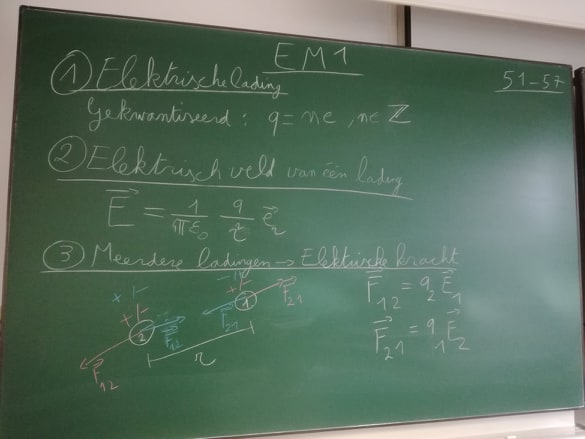
\includegraphics[width=0.9\textwidth]{Bord1a}
%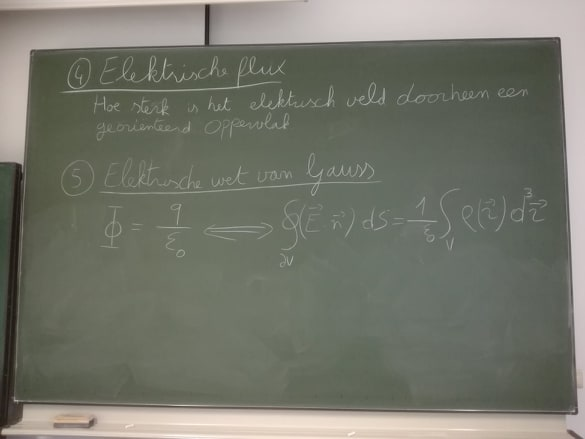
\includegraphics[width=0.9\textwidth]{Bord1b}
%\end{center}
%\newpage
%
%
%\includepdf[scale = 0.8,pages = 17,pagecommand=\subsection*{Bijlage 1.3: opgeloste oefeningen}]{Observaties_OpgelosteOef}
%\includepdf[scale = 0.8,pages =18-20,pagecommand=]{Observaties_OpgelosteOef}
%
%
%
%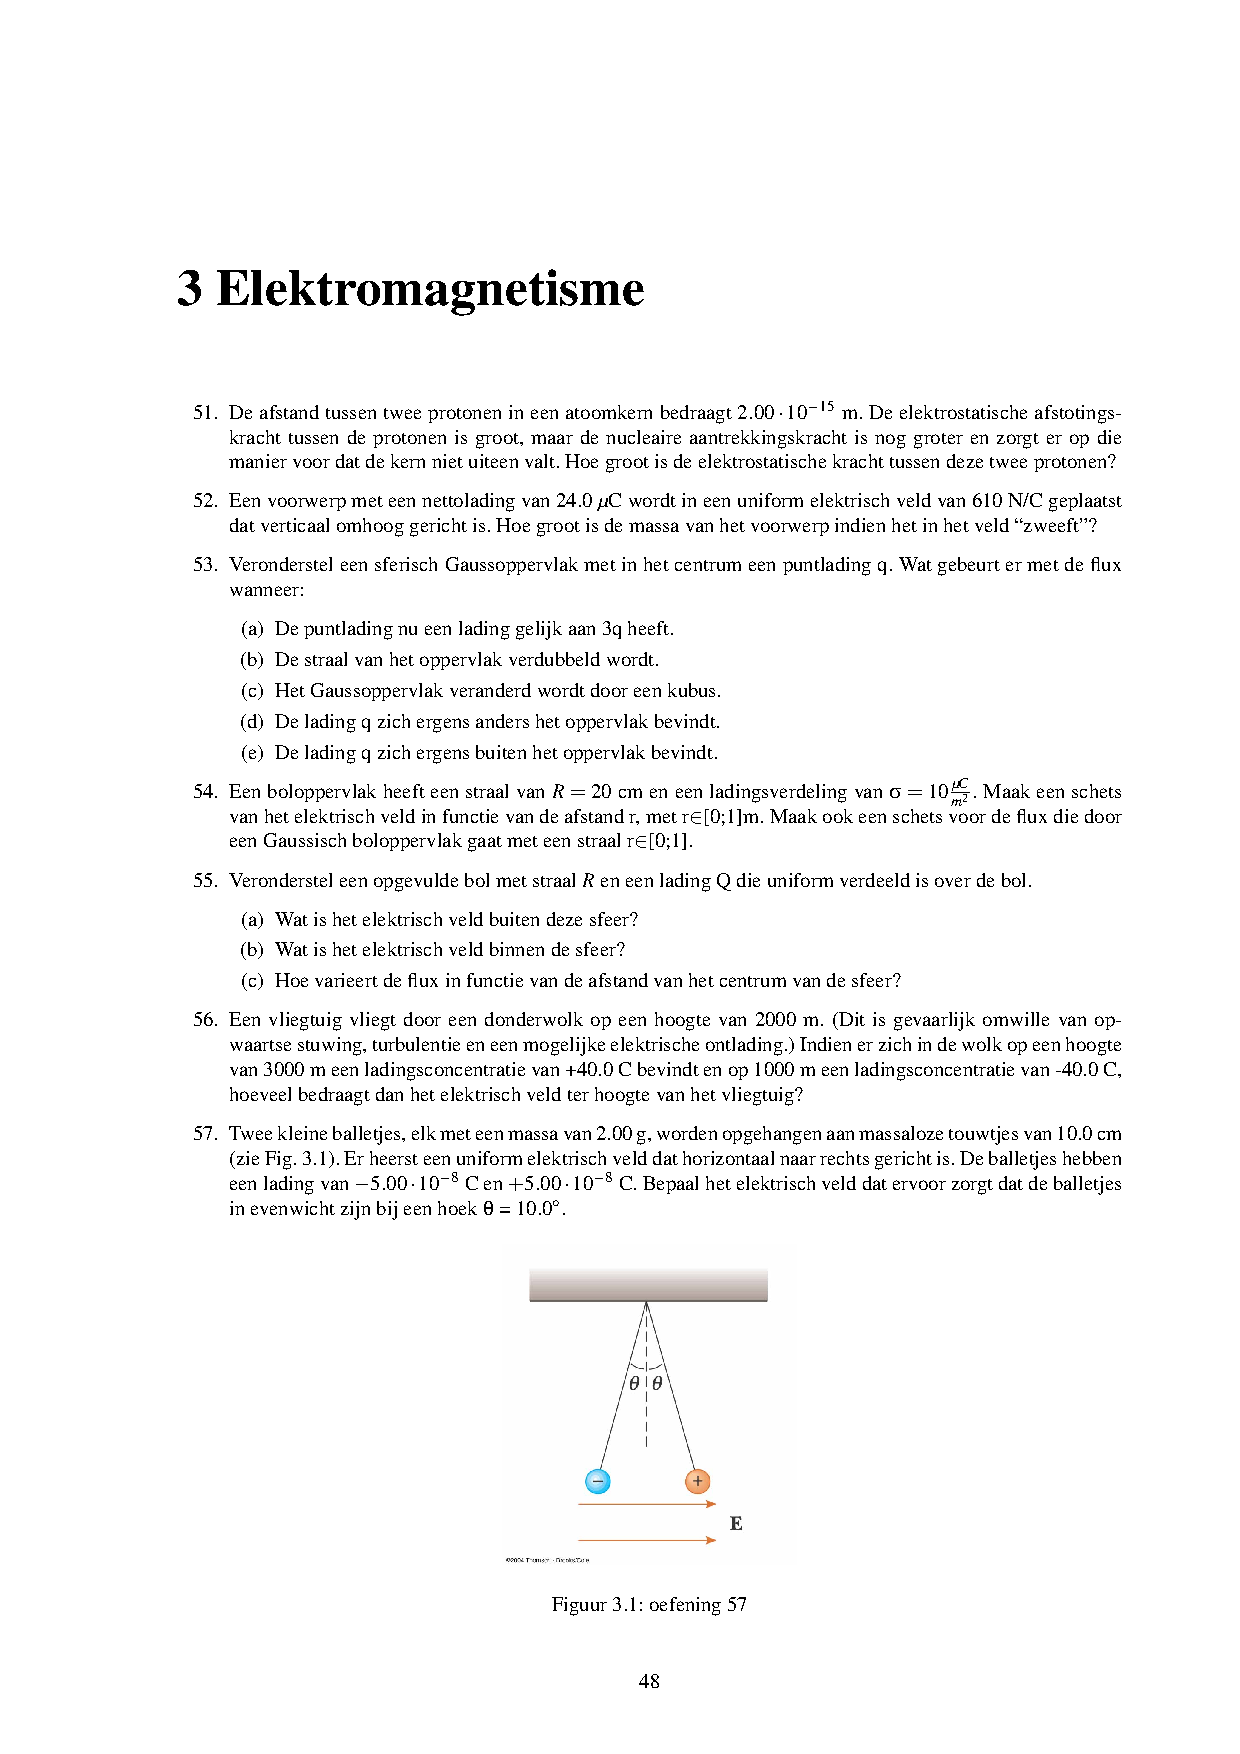
\includepdf[scale = 0.95,pages = 1,pagecommand=\subsection*{Bijlage 1.4: oefeningenbundel elektromagnetisme}]{OefeningenBundel}
%\includepdf[scale = 0.95,pages =2-,pagecommand=]{OefeningenBundel}